\documentclass[conference]{IEEEtran}
%\renewcommand{\thesubsection}{\thesection.\alph{subsection}}
\renewcommand{\floatpagefraction}{.8}%
%\addtolength{\oddsidemargin}{-.875in}
%\addtolength{\evensidemargin}{-.875in}
%\addtolength{\textwidth}{1.75in}
%\addtolength{\topmargin}{-.875in}
%\addtolength{\textheight}{1.75in}
	
\usepackage{bm}
\usepackage{amsmath}
\usepackage{amssymb}
\usepackage{tikz}
\usetikzlibrary{automata,positioning}
\usepackage{url}
\usepackage{float}
\usepackage{setspace}
\usepackage{filecontents,lipsum}
\usepackage[noadjust]{cite}
\usepackage{listings}
\usepackage{caption}


\begin{document}
%\raggedright
%\doublespacing

\title{Research Proposal for Code Smell Algorithm Training Dataset Analysis}
\author{Rodger Byrd\\rbyrd2@uccs.edu}
\maketitle

\section{Introduction to the Problem}
This proposal is for research involving machine learning and code smells.
A lot of previous research has been done on the performance of different algorithms and the detecting of different subsections of code smells.
This paper will focus on training datasets with regard to machine learning and code smells. 
Many different approaches have been taken with regards to training datasets, but they haven't been compared for effectiveness in training the machine learning algorithms.


A code smell is a description of a pattern in code that might cause deeper problems. 
Code smells are not easily found and can vary by programming language and development methodoligies.
The existence of code smells and antipatterns implies that there are potential problems with software sustainment and imply there are issues with the design.
Kent Beck coined the term ``code smell'' \cite{fowler_refactoring:_2018} and defined as ``certain structures in the code that suggest (sometimes they scream for) the possibility of refactoring''.
Machine learning is defined as computers learning to solve problems without being explicitly programmed, although they are ``trained''\cite{bishop_pattern_2006}. 
Arthur Samuel coined the term Machine Learning in 1959\cite{samuel_studies_1988}.


Machine learning is a subset of artificial intelligence. 
It uses algorithms and statistical models to execute a task without explicitly being programmed.
Machine learning is used in a wide variety of applications such as email spam filtering, search engines, video surveillance, and image curation.


A big challenge in this field determining the best way to identify code smells and how training datasets are labeled and created.
There is a lot of inconsistency in training datasets and identifying code smells because they can be subjectively interpreted.
Additionally, expert advice and knowledge may be able to help identify code smells, using it to train datasets may not be effective unless it has been experimentally shown to be result in finding code smells. 

It is difficult to compare the results of previous research due to the variability of training datasets and differences in machine learning algorithms.
This research will compare training datasets and code smell definitions for performance.

Figure \ref{fig:ts} show the "potential" results of comparison by algorithm. 

There are many existing public training datasets that can be compared such as the research performed by Fontana et al.\cite{arcelli_fontana_comparing_2016} 
The different studies comparing machine learning performance with regard to code smells vary, and don't all study the same smells.

\begin{center}
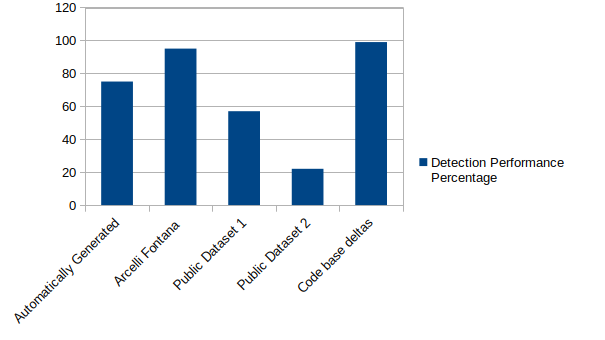
\includegraphics[width=\columnwidth]{teaser.png}
\captionof{figure}{Training Data Performance}\label{fig:ts}%
\end{center}

%\begin{figure*}[ht]{
% 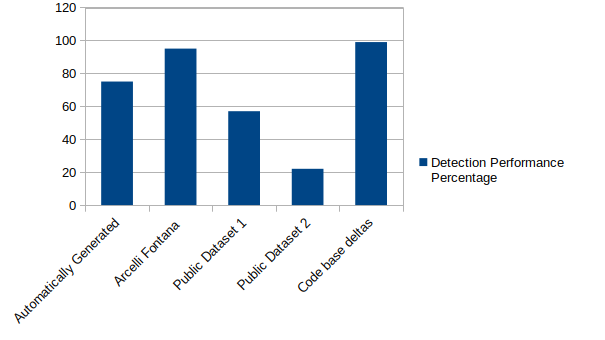
\includegraphics[width=\columnwidth]{teaser.png}}
%  \caption{Training Data Performance}
%  \label{fig:ts}
%\end{figure*} 

\section{The Approach}
The approach to this research will be to compare training datasets for performance in detecting code smells.
Common existing public datasets will be compared using the highest performing algorithms to determine which has the best performance.

\section{Experimental Design}
%A formal section on Experimental Design and datasets 
The experiment will test accuracy on performace of algorithms using different training dataset approaches.
The following approaches to creating training datasets are: 
\begin{enumerate}
\item datasets created by software experts
\item datasets created by performing a survey of software developers 
\item datasets used in other published experiments
\item automated dataset generation
\item using public code base changes to identify code corrections and the implied code smells
\end{enumerate}
A single machine learning algorithm will be used for all testing. 
From previousl research\cite{arcelli_fontana_comparing_2016}, the J48 and Random Forest algorithms are the highest performing when compared against other algorithms using the same training data.
%how to use more than one algorithm
The experiment will compare perfomance in correctly identifying code smells and the type of smells that can be identified. 
An example table is shown in figure \ref{fig:acc}.

\begin{center}
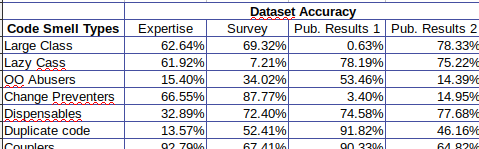
\includegraphics[width=\columnwidth]{performance.png}
\captionof{figure}{Training Data Accuracy}\label{fig:acc}%
\end{center}

A second part of the research will be to see if the training datasets can be optimized and improved based off of the first part of the experiment.

\section{Hypothesis and Stastical Testing}
%A formal section on the hypothesis and Statistical Testing for that hypothesis for your given design and the outcomes of the experiments.
\subsection{Hypothesis}
There are a few hypothesis to test:
\begin{enumerate}

\item Training datasets will have varying performance
\item They can more accurately identify code smells and identify a broader set of code smell types
\item Datasets can be optimized and improved

\end{enumerate}
\subsection{Stastical Testing}
Statistical testing will be performed by comparing training datasets with regards to their behavior and coverage.

T-tests will be performed to determine if the results from the research is significant, and if so, by how much. Results will be provided, an example is provided in figure \ref{fig:stat}.
\begin{center}
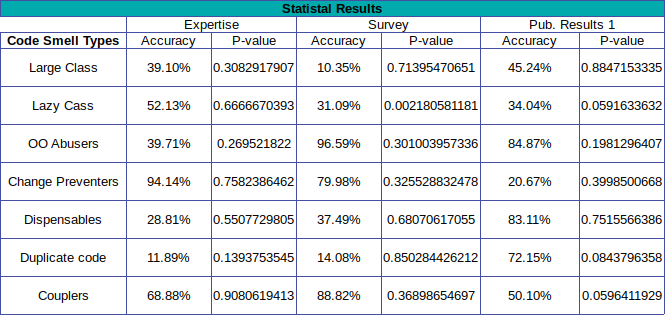
\includegraphics[width=\columnwidth]{statistics.png}
\captionof{figure}{Test Results}\label{fig:stat}%
\end{center}

\section{Research Plan and Timeline}
Beginning Fall 2019 the project milestones are identified in figure \ref{fig:sch}.
\begin{center}
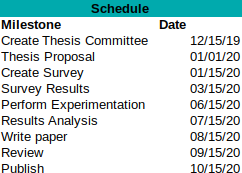
\includegraphics[width=\columnwidth]{schedule.png}
\captionof{figure}{Schedule}\label{fig:sch}%
\end{center}

Scope and schedule may need to change as the research project progresses.
%Relevan papers are referenced in the bibliography below. 
%\nocite{*}
%\clearpage


\bibliographystyle{IEEEtran}
\bibliography{references}


\end{document}